\documentclass{crypto-exercise}
\usepackage{float}
\author{Sven Laur}
\editor{Sven Laur}
\tags{Turing machine, Random Access Machine, program hardwiring}

\newcommand{\PRINT}{\textbf{print }}

\begin{document}

\begin{exercise}{On the necessity of universality}
Let $\GG$ be a finite group such that all elements $y \in \GG$ can be expressed
as powers of $g \in \GG$. Then the discrete logarithm problem is following.
Given $y \in \GG$, find a smallest integer $x$ such that $g^x = y$ in finite group
$\GG$. Discrete logarithm problem is known to be hard in general, i.e., all
universal algorithms for computing logarithm run in time $\Omega(\sqrt{|\GG|})$.
\begin{enumerate}
\item[(a)] Show that for a fixed group $\GG$, there exists a Turing machine that
finds the discrete logarithm for every $y \in \GG$ in $\Theta(\log_2 |\GG|)$ steps.
\item[(b)] Show that for a fixed group $\GG$, there exists an analogous Random
Access Machine that achieves the same efficiency.
\item[(c)] Generalise the previous construction and show that for every fixed
function $f : \set{0, 1 } ^n \to \set{0, 1}^m$ there exists a Turing machine and
a Random Access Machine such that they compute $f(x)$ for every
input $x \in \set{0, 1 }^n$ in $O(n + m)$ steps.
\item[(d)] Are these constructions also valid in practise? Explain why these
inconsistencies disappear when we formalise algorithms through universal computing devices. 
\end{enumerate}
\end{exercise}
\begin{solution}
\textsc{Hardwired Turing Machine.}
Let us consider a group $\GG$ of size $q$. Since the group is fixed, we can create the following table containing all possible powers.
\begin{center} 
\begin{tabular}{|l|c|c|c|c|}
\hline
Power $x$ & $0$ & $1$ & $\ldots$ & $q-1$\\
\hline
Result $g^x$ & $1$ & $g$ & $\ldots$ & $g^{q-1}$\\
\hline
\end{tabular}
\end{center}
By reordering the columns lexicographically according to the exponentiation results, we get similar lookup table for discrete logarithm. 
\begin{center} 
\begin{tabular}{|l|c|c|c|c|}
\hline
Result $g^x$ & $0\ldots0_2$ & $0\ldots1_2$ & $\ldots$ & $1\ldots1_2$\\
\hline
Power $x$ & $\log(0\ldots0_2)$ & $\log(0\ldots1_2)$ & $\ldots$ & $\log(1\ldots1_2)$\\
\hline
\end{tabular}
\end{center}
As a concrete example consider an eight element group with the following discrete logarithm table
\begin{center} 
\begin{tabular}{|l|c|c|c|c|c|c|c|c|}
\hline
Result $g^x$ & $000_2$ & $001_2$ & $010_2$ & $011_2$ & $100_2$ & $101_2$ & $110_2$ & $111_2$\\
\hline
Power $x$ &  $111_2$ & $101_2$ & $110_2$ & $100_2$ & $011_2$ & $001_2$ & $010_2$ & $000_2$\\
\hline
\end{tabular}
\end{center}
Now given this table it is straightforward to output the correct result by comparing the input $x$ to the label of the first column, to label of the second column and so on until we have a match and then output the corresponding discrete logarithm value. However, this algorithm makes $q/2$ comparisons on the average. By using binary search it is easy to reduce the number of comparisons to $\ceil{\log q}$. More precisely, we can represent the search as a traversal of full binary tree where in the $i^{\text{th}}$ level node we choose the left child if the $i^{\text{th}}$ input bit is zero and the right node if the $i^{\text{th}}$ input bit is one. For our toy example, the corresponding traversal scheme is depicted in Figure~\ref{fig:binary-tree-traversal}. As the next step towards the Turing machine, we assign the start state $q_{0\ldots0}$ to the root of the tree and distinct states $q_i$ for the remaining states. As a result, we get a pictorial description of the state transitions in the Turing machine we are going to construct. Figure~\ref{fig:state-diagram}. The diagram is incomplete in the sense that after we reach the leaf state we should print out the corresponding answer and put the reading head to the right position. For any fixed output $y$, the corresponding program fragment in Turing machine is a simple straight line program. For example, the following program fragment outputs $010_2$ and returns the reading head in front of it.
\begin{center}
\begin{tabular}{|c|c|c|c|c|}
\hline
 State & -- & $0$ & $1$\\
 \hline
 $q_{000}$ &--$q_{001}$R & 0$q_{001}$R & 1$q_{001}$R \\ 
 $q_{001}$ & 0$q_{010}$R & 0$q_{010}$R & 0$q_{010}$R \\ 
 $q_{010}$ & 1$q_{011}$R & 1$q_{011}$R & 1$q_{011}$R \\ 
 $q_{011}$ & 0$q_{100}$R & 0$q_{100}$R & 0$q_{100}$R \\ 
 $q_{100}$ &--$q_{end}$C & 0$q_{100}$L & 1$q_{100}$L \\ 
\hline
\end{tabular}
\end{center}           
Hence, if we encode the pictorial description of state transitions corresponding to the binary search of the right index and in each leaf node forward the execution to the straight line program printing the answer, we get a turing machine with $\Theta(q)$ states that for any input makes $\ceil{\log q}$ steps to reach the leaf state in the binary search and then makes additionally $\Theta(\log q)$ steps to print out the answer and take the machine into correct end state. Thus, we have constructively proved that for any group $\GG$ there exists a Turing machine that correctly computes discrete logarithm in $\Theta(\log q)$ steps.    

\begin{figure}
\centerline{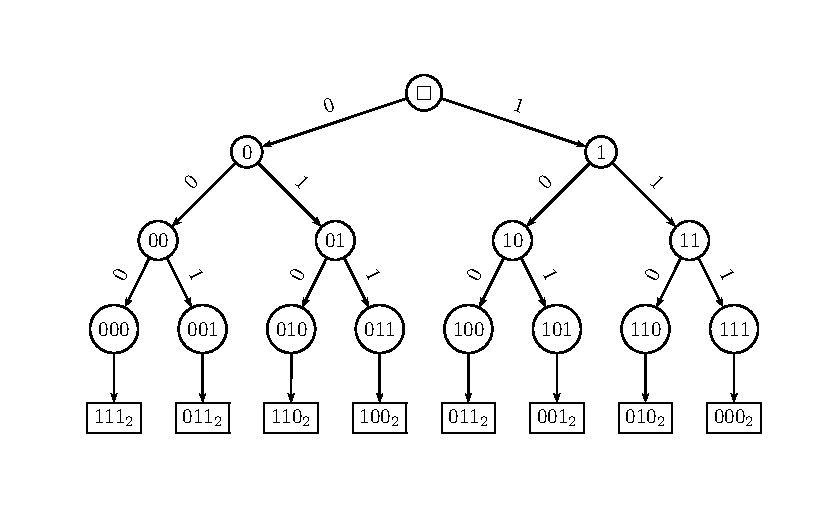
\includegraphics[trim=1cm 1cm 1cm 1cm, clip]{figures/input-tree}}
\caption{Binary decision tree corresponding to discrete logarithm evaluation}
\label{fig:binary-tree-traversal}
\end{figure}
\begin{figure}[!h]
\centerline{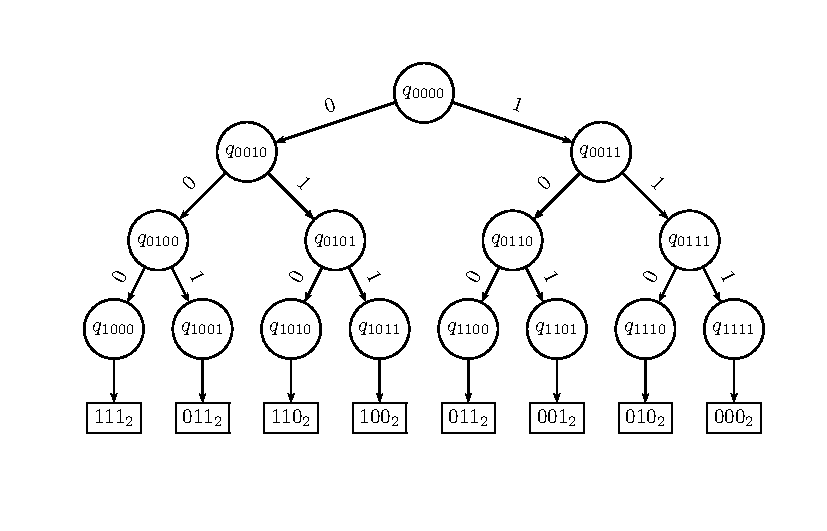
\includegraphics[trim=1cm 1cm 1cm 1cm, clip]{figures/state-tree}}
\caption{State transition diagram for the Turing machine with initial state $q_{0000}$}
\label{fig:state-diagram}
\end{figure}

\vspace*{2ex}
\noindent\textsc{Hardwired Random Access Machine.}
As a RAM machine code contains conditional jump instructions and thus implementing state traversal is a straightforward task. For instance, we can first read the $i^{\text{th}}$ bit to the register \texttt{R} and then use \mbox{\texttt{JMPZ R, PC}} instruction to implement branching. Recall that mbox{\texttt{JMPZ R, PC}} sets the program counter to the value \texttt{PC} if the register \texttt{R} is zero and otherwise it just fetches the next instruction. Note that the naive solution, which would first write $\log(0\ldots0_2)$ to the register $R_0$, $\log(0\ldots1_2)$ to the register $R_1$ and so on and then use simple addressing command \texttt{PRINT R[$x$]} for input $x$, is not efficient as the time needed to build the table is $\Omega(q)$. It is really important that the search for the answer is encoded into the program code itself, as standard timing models neglect the time needed to load the code.    

\vspace*{2ex}
\noindent\textsc{Generalisation to any function.}
The steps we did for construction of the discrete logarithm finder can be used for any function. First, we should construct the input output table for the function. Based on that we can construct the similar state transformation tree where the leafs will link to straight-line programs that print the desired outputs. As the construction is analogous, the execution will take $\Theta(n+m)$ steps as required. The similar reasoning holds also for the RAM model.
 
\vspace*{2ex}
\noindent\textsc{Real-life limitations.} 
All constructions described above have exponential number of states. This leads to two kinds of problems. First, someone has to write this program and by using current technology this procedure itself would take humongous amount of time. However, such a construction is not feasible even if we assume that a super-powerful entity builds the machine for us. Since the number of states is exponential, it also takes exponential number of electronic elements to encode the table. As all such elements are physical objects with finite size then the entire equipment must take a large volume. During the program execution we have to be able access large fraction of states. Since the equipment has a large volume, the distance between states is also large. As a consequence from special relativity theory, the information fetching must be slow. We can roughly estimate that it takes at least $\Omega(\sqrt[3]{2^{n}})$ for some transition.

\end{solution}
\end{document}
